

\documentclass[journal]{IEEEtran}
\usepackage{tablefootnote}
% Some Computer Society conferences also require the compsoc mode option,
% but others use the standard conference format.
%
% If IEEEtran.cls has not been installed into the LaTeX system files,
% manually specify the path to it like:
% \documentclass[conference]{../sty/IEEEtran}





% Some very useful LaTeX packages include:
% (uncomment the ones you want to load)


% *** MISC UTILITY PACKAGES ***
%
%\usepackage{ifpdf}
% Heiko Oberdiek's ifpdf.sty is very useful if you need conditional
% compilation based on whether the output is pdf or dvi.
% usage:
% \ifpdf
%   % pdf code
% \else
%   % dvi code
% \fi
% The latest version of ifpdf.sty can be obtained from:
% http://www.ctan.org/pkg/ifpdf
% Also, note that IEEEtran.cls V1.7 and later provides a builtin
% \ifCLASSINFOpdf conditional that works the same way.
% When switching from latex to pdflatex and vice-versa, the compiler may
% have to be run twice to clear warning/error fsages.






% *** CITATION PACKAGES ***
%
%\usepackage{cite}

% cite.sty was written by Donald Arseneau
% V1.6 and later of IEEEtran pre-defines the format of the cite.sty package
% \cite{} output to follow that of the IEEE. Loading the cite package will
% result in citation numbers being automatically sorted and properly
% "compressed/ranged". e.g., [1], [9], [2], [7], [5], [6] without using
% cite.sty will become [1], [2], [5]--[7], [9] using cite.sty. cite.sty's
% \cite will automatically add leading space, if needed. Use cite.sty's
% noadjust option (cite.sty V3.8 and later) if you want to turn this off
% such as if a citation ever needs to be enclosed in parenthesis.
% cite.sty is already installed on most LaTeX systems. Be sure and use
% version 5.0 (2009-03-20) and later if using hyperref.sty.
% The latest version can be obtained at:
% http://www.ctan.org/pkg/cite
% The documentation is contained in the cite.sty file itself.






% *** GRAPHICS RELATED PACKAGES ***
%
\ifCLASSINFOpdf
\usepackage{graphicx}

\usepackage{booktabs} % lluis added these:
\usepackage{multirow}
\usepackage{siunitx}
  % \usepackage[pdftex]{graphicx}
  % declare the path(s) where your graphic files are
  % \graphicspath{{../pdf/}{../jpeg/}}
  % and their extensions so you won't have to specify these with
  % every instance of \includegraphics
  % \DeclareGraphicsExtensions{.pdf,.jpeg,.png}
\else
  % or other class option (dvipsone, dvipdf, if not using dvips). graphicx
  % will default to the driver specified in the system graphics.cfg if no
  % driver is specified.
  % \usepackage[dvips]{graphicx}
  % declare the path(s) where your graphic files are
  % \graphicspath{{../eps/}}
  % and their extensions so you won't have to specify these with
  % every instance of \includegraphics
  % \DeclareGraphicsExtensions{.eps}
\fi
% graphicx was written by David Carlisle and Sebastian Rahtz. It is
% required if you want graphics, photos, etc. graphicx.sty is already
% installed on most LaTeX systems. The latest version and documentation
% can be obtained at: 
% http://www.ctan.org/pkg/graphicx
% Another good source of documentation is "Using Imported Graphics in
% LaTeX2e" by Keith Reckdahl which can be found at:
% http://www.ctan.org/pkg/epslatex
%
% latex, and pdflatex in dvi mode, support graphics in encapsulated
% postscript (.eps) format. pdflatex in pdf mode supports graphics
% in .pdf, .jpeg, .png and .mps (metapost) formats. Users should ensure
% that all non-photo figures use a vector format (.eps, .pdf, .mps) and
% not a bitmapped formats (.jpeg, .png). The IEEE frowns on bitmapped formats
% which can result in "jaggedy"/blurry rendering of lines and letters as
% well as large increases in file sizes.
%
% You can find documentation about the pdfTeX application at:
% http://www.tug.org/applications/pdftex


\usepackage{scrextend} % mg added this. use the same footnote mark 
\usepackage{gensymb}

% *** MATH PACKAGES ***
%
\usepackage{amsmath}
%\usepackage{breqn}


% *** SPECIALIZED LIST PACKAGES ***
%
%\usepackage{algorithmic}




% *** ALIGNMENT PACKAGES ***
%
%\usepackage{array}


% *** SUBFIGURE PACKAGES ***
%\ifCLASSOPTIONcompsoc
%  \usepackage[caption=false,font=normalsize,labelfont=sf,textfont=sf]{subfig}
%\else
%  \usepackage[caption=false,font=footnotesize]{subfig}
%\fi
% subfig.sty, written by Steven Douglas Cochran, is the modern replacement
% for subfigure.sty, the latter of which is no longer maintained and is
% incompatible with some LaTeX packages including fixltx2e. However,
% subfig.sty requires and automatically loads Axel Sommerfeldt's caption.sty
% which will override IEEEtran.cls' handling of captions and this will result
% in non-IEEE style figure/table captions. To prevent this problem, be sure
% and invoke subfig.sty's "caption=false" package option (available since
% subfig.sty version 1.3, 2005/06/28) as this is will preserve IEEEtran.cls
% handling of captions.
% Note that the Computer Society format requires a larger sans serif font
% than the serif footnote size font used in traditional IEEE formatting
% and thus the need to invoke different subfig.sty package options depending
% on whether compsoc mode has been enabled.
%
% The latest version and documentation of subfig.sty can be obtained at:
% http://www.ctan.org/pkg/subfig




% *** FLOAT PACKAGES ***
%
%\usepackage{fixltx2e}
% fixltx2e, the successor to the earlier fix2col.sty, was written by
% Frank Mittelbach and David Carlisle. This package corrects a few problems
% in the LaTeX2e kernel, the most notable of which is that in current
% LaTeX2e releases, the ordering of single and double column floats is not
% guaranteed to be preserved. Thus, an unpatched LaTeX2e can allow a
% single column figure to be placed prior to an earlier double column
% figure.
% Be aware that LaTeX2e kernels dated 2015 and later have fixltx2e.sty's
% corrections already built into the system in which case a warning will
% be issued if an attempt is made to load fixltx2e.sty as it is no longer
% needed.
% The latest version and documentation can be found at:
% http://www.ctan.org/pkg/fixltx2e


%\usepackage{stfloats}
% stfloats.sty was written by Sigitas Tolusis. This package gives LaTeX2e
% the ability to do double column floats at the bottom of the page as well
% as the top. (e.g., "\begin{figure*}[!b]" is not normally possible in
% LaTeX2e). It also provides a command:
%\fnbelowfloat
% to enable the placement of footnotes below bottom floats (the standard
% LaTeX2e kernel puts them above bottom floats). This is an invasive package
% which rewrites many portions of the LaTeX2e float routines. It may not work
% with other packages that modify the LaTeX2e float routines. The latest
% version and documentation can be obtained at:
% http://www.ctan.org/pkg/stfloats
% Do not use the stfloats baselinefloat ability as the IEEE does not allow
% \baselineskip to stretch. Authors submitting work to the IEEE should note
% that the IEEE rarely uses double column equations and that authors should try
% to avoid such use. Do not be tempted to use the cuted.sty or midfloat.sty
% packages (also by Sigitas Tolusis) as the IEEE does not format its papers in
% such ways.
% Do not attempt to use stfloats with fixltx2e as they are incompatible.
% Instead, use Morten Hogholm'a dblfloatfix which combines the features
% of both fixltx2e and stfloats:
%
% \usepackage{dblfloatfix}
% The latest version can be found at:
% http://www.ctan.org/pkg/dblfloatfix

% \usepackage[backend=biber]{biblatex}      %backend=biber: si dice a biblatex che si intende usare biber come motore bibliografico



% *** PDF, URL AND HYPERLINK PACKAGES ***
%

\usepackage[hyphens]{url}
% url.sty was written by Donald Arseneau. It provides better support for
% handling and breaking URLs. url.sty is already installed on most LaTeX
% systems. The latest version and documentation can be obtained at:
% http://www.ctan.org/pkg/url
% Basically, \url{my_url_here}.






% correct bad hyphenation here
\hyphenation{op-tical net-works semi-conduc-tor}


\begin{document}
%
% paper title
% Titles are generally capitalized except for words such as a, an, and, as,
% at, but, by, for, in, nor, of, on, or, the, to and up, which are usually
% not capitalized unless they are the first or last word of the title.
% Linebreaks \\ can be used within to get better formatting as desired.
% Do not put math or special symbols in the title.
\title{An efficient 3-D sound experience for mobile applications}


% author names and affiliations
% use a multiple column layout for up to three different
% affiliations
\author{\IEEEauthorblockN{Group 3}
\IEEEauthorblockA{
Aalborg University\\
Copenhagen, Denmark\\
}}


% conference papers do not typically use \thanks and this command
% is locked out in conference mode. If really needed, such as for
% the acknowledgment of grants, issue a \IEEEoverridecommandlockouts
% after \documentclass

% for over three affiliations, or if they all won't fit within the width
% of the page, use this alternative format:
% 
%\author{\IEEEauthorblockN{Michael Shell\IEEEauthorrefmark{1},
%Homer Simpson\IEEEauthorrefmark{2},
%James Kirk\IEEEauthorrefmark{3}, 
%Montgomery Scott\IEEEauthorrefmark{3} and
%Eldon Tyrell\IEEEauthorrefmark{4}}
%\IEEEauthorblockA{\IEEEauthorrefmark{1}School of Electrical and Computer Engineering\\
%Georgia Institute of Technology,
%Atlanta, Georgia 30332--0250\\ Email: see http://www.michaelshell.org/contact.html}
%\IEEEauthorblockA{\IEEEauthorrefmark{2}Twentieth Century Fox, Springfield, USA\\
%Email: homer@thesimpsons.com}
%\IEEEauthorblockA{\IEEEauthorrefmark{3}Starfleet Academy, San Francisco, California 96678-2391\\
%Telephone: (800) 555--1212, Fax: (888) 555--1212}
%\IEEEauthorblockA{\IEEEauthorrefmark{4}Tyrell Inc., 123 Replicant Street, Los Angeles, California 90210--4321}}


% *****************************************************************************************************
% *****************************************************************************************************
% added by mg. it is the structure that Stefania suggested use to use
% THIS SHOULD BE THE MAIN STRUCTURE OF THE PAPER
% Here is the structure
% 1) Abstract: a summary of the project and results
% 2) Introduction: Your problem, state of the art
% 3) Implementation: description of your app, the 3D sound features, the sounds,etc….
% 4) Experiment design
% -description of experiment
% -data analysis
% -discussion
% 5) Conclusion 
% -your conclusion
% future work
% -references
% Appendix
% with implementations, etc….all you did which does not fit inside the paper
% *****************************************************************************************************
% *****************************************************************************************************

% use for special paper notices
%\IEEEspecialpapernotice{(Invited Paper)}
% The paper headers

\markboth{Journal of \LaTeX\ Class Files,~Vol.~11, No.~4, December~2012}%
{Shell \MakeLowercase{\textit{et al.}}: Bare Demo of IEEEtran.cls for Journals}
% The only time the second header will appear is for the odd numbered pages
% after the title page when using the twoside option.
% 
% *** Note that you probably will NOT want to include the author's ***
% *** name in the headers of peer review papers.                   ***
% You can use \ifCLASSOPTIONpeerreview for conditional compilation here if
% you desire.




% If you want to put a publisher's ID mark on the page you can do it like
% this:
%\IEEEpubid{0000--0000/00\$00.00~\copyright~2012 IEEE}
% Remember, if you use this you must call \IEEEpubidadjcol in the second
% column for its text to clear the IEEEpubid mark.



% use for special paper notices
%\IEEEspecialpapernotice{(Invited Paper)}




% make the title area
\maketitle

% As a general rule, do not put math, special symbols or citations
% in the abstract
\begin{abstract}

\\ \textit{previous version}\\
We developed an application for mobile devices that uses an efficient HRTF model based on to create 3D soundscapes. The HRTF model is based on a combination of filters and delays provided on theoretical basis by Brown et. al. [1]. The device orientation is used to set the angle between the sound and the user. This model has many possibilities on the limited hardware capabilities of the mobile devices in comparison to HRTF database based models. The prototype will present the user several sounds scattered in a limited area where the user can interact with.

{\textit{matteo's version}}\\
Since the calculating capacity of mobile devices has highly increased in the last few years and almost every device has a GPS/compass sensor, it is now possible to enhance the user daily life experience. The main issue is how much can an HRTF model improve the user experience of hearing sound through headphones. Therefore an efficient HRTF model based on~\cite{Brown1997} has been implemented, and combining it with sensors data such as those stated above, it is possible to place a `virtual sound object' in a specific location. Additionaly, the required angle between the sound and the user is computed. The user can therefore explore an environment through sound. To test our hypothesis the HRTF model is compared with a cosine panner model~\cite{AndyFarnell2010}. write the results and the conclusion.
\end{abstract}


% Note that keywords are not normally used for peerreview papers.
\begin{IEEEkeywords}
HTRF, mobile devices, soundscape, Pure Data, OpenFrameworks
\end{IEEEkeywords}



\section{Introduction}

A lot of research on modeling 3-D sound has been done with fairly good results~\cite{begault19943}. The best results can be obtained by those models implementing 3-D sound using personalized Head related transfer functions (HRTF) which needs tedious measuring of impulse responses etc. ~\cite{Meshram2014}. Mobile applications as well as multimedia productions are usually aimed at a big number of users, thus implementing HRTFs requiring measurements of the individual user would be very inpractcal. Furthermore the convolution needed for using databases with Head related impulse responses is an unnessesarry heavy technique in terms of computational power and memory, two things that are not abundand in mobile devices. Therefore, the aim of this project was to develop a computationally efficient and general HRTF model, yet, keeping the quality of the 3-D sound as good as possible. We used the model provided on a theoretical basis in~\cite{Brown1997} by implementing a combination of filters and delays in Pure Data and C. This audio engine was then embedded in a mobile application. Compass and GPS data provided by the mobile device was used to compute from which direction and at what distance the sound should appear to be coming from. With the application users should be able to discover a virtual sound space situated in Copenhagen. our HRTF model should satisfy two major requirements. 
\\1. It should provide direction cues that are good enough to guide the user to the position where a specific sound is situated.\\2. The implemented HRTF model should provide an intuitive way of locating a sound source from an qualitative aspect. \\The first aim was to let the user find a sound source as fast as possible hypothesizing that our model would give and better or at least as good result as a simple stereophonic panning. Our second hypothesis was that the model would give a qualitatively more natural and intuitive feeling of the sounds position in the space

Taken both hypothesizes together the user should experience a soundscape in at least 2-dimensions, azimuth and distance.

The purpose of this paper is first to describe the implementation of a efficient and general HRTF model for mobile devices. Secondly to make a comparative test between that and a simple stereophonic panning based on both qualitative and quantitative measures. 

First, some state of the art research on audio augmented reality will be provided. That section will be followed by the presentation of our implementation of the audio engine as well as the main application. In the last part we will present the results obtained by testing our application and discuss those in light of the two hypotheses stated above.



\subsection{State of the art}
The concept of audio augmented reality (AAR) deals with techniques where a real sound environment is extended with virtual auditory environments. Recently, the progress in audio technology and computing predicts the introduction of completely new type of interactive audio applications~\cite{}. Advances in mobile technologies have made it possible to create audio augmented spaces almost anywhere. For instance, spatial auditory displays that can provide the user with landmarks and are capable to attract the user's attention have been tested and introduced~\cite{}. Many experiments, qualitative and quantitative researches have been designed so far to better understand the way in which people usually perceive multiple simultaneous sources differently placed and to increase the level of immersion in the experience.

\subsubsection{Audio reality vs Augmented reality}
First of all, the possibility to hear the natural acoustic environment around a user differentiates the concept of audio augmented reality from the traditional concept of a virtual reality audio environment~\cite{}. In virtual reality, generally participants are abstracted from the natural environment and are surrounded only by a completely synthetic one (acoustic and/or visual). On the opposite, in augmented reality a virtual environment is \emph{superimposed} on a real one. To be more specific, in a mobile audio augmented environment participants are able to interact with the virtual audio mixed with real vision and/or soundscape.

\subsubsection{Augmented audio reality}
taking this definition of augmented reality, audio audmente reality (AAR) should be within the bounderies of 1) a perfect augmentation of the listener's auditory environment and is achieved when the listener is unable to predict whether a sound source is part of the real or the virtual audio environment.and 2) a set of artifisial sounds that are not possiblein the real world sumperimposed and fitted to the visual percieved world like in \cite{}. Any combination of these two fall within the boundaries of AAR

\subsubsection{Previous work}
Several work has been done in this field although this area is relatively new. \emph{Audio Aura} (Mynatt 1995) was one of the first project to deal exclusively with audio in augmented reality system. It basically consisted in providing information to users as they travelled through their workspace. These information was triggered by particular locations in the workspace. The use of audio in \emph{Audio Aura} is particularly interesting because most of its cues were associated to sounds from nature rather then recorded vocal, speech or synthetic sounds. Similar in approach to \emph{Audio Aura} was the \emph{Automated Tour Guide} (Bederson 1995). In both cases, triggers are readily identifiable, still and rarely changing. Those augmented sounds were associated to pre-determined locations in space and there was no need to determine the precise location of an individual. \\
A successive work, \emph{Hear\&There}, was able to determine the location and head position of the user using the information from GPS and a digital compass~\cite{}. A user could listen to these `audio imprints` by walking into the area that a specific imprint occupied, which was triggered by proximity. The essential premise of  \emph{Hear\&There} was that a physical environment has been augmented with audio. All the sounds and the data were gathered inside that system. Since a `Field Use` has been developed, in which the user wear a hardware portable system, \emph{Hear\&There} has undoubtedly contributed to an improved definition of mobile augmented reality environment.

\subsubsection{Human sound localization}
The auditory system is used by the humans for several purposes in the daily life. One of this purposes is to provide the necessary information to localize sound sources in various dimensions, (width, height, depth) and it is even possible to guess the size of the source.\\

When a sound event   occurs,   the   waves   travel   in   all directions and ,  when  they  reach  us,  our  brain  compares  the signals  received  by  the  left  and  right  ears  to  localize  it in the horizontal plane.  The spectrum of the signal reaching each ear is different, since the amplitude and phase information differs. These binaural cues are  called  \emph{interaural  intensity  difference}  (IID)  and  \emph{interaural time  difference}  (ITD). However, these cues are not enough to localize accurately the source since with this information the listener can not determine if the sound is in front, above or behind. This region of positions where all sounds yield the same ITD and IID is called \textit{cone of confusion}.
This ambiguity can be solved with the information provided by the filter effect caused by the pinnae, head, shoulders and torso, which modify the spectrum of the sound that reach the listener's ears. The sum of all these features are characterized by the Head Related Transfer Functions (HTRF) which are not only frequency and direction-dependent but also differ from person to person. That dependency makes therefore hard to generalize the spectral features among individuals. It is well known that using a HTRF from one person in another can significantly impair the  perception due to the individual differences in the anatomy, but it has also been shown that some people localize better the sounds than others, and their HTRFs are suitable for a large group of listeners.

%Thus, having a database with own measured HRTF for each user would be the ideal case. However, because of the large amount of data that the customized HTRFs required to generate externalized virtual sources would entail, and the expensive real-time computation of them every time the sound source moves, this is almost impossible. In addition, due to the limited memory space of the mobile devices, having a database with standard HTRFs would not be the best choice and it is desirable to find a more efficient HTRF model.\\

\subsubsection{Localization/Lateralization}
Headphones are an intergraded part of many mobile and wearable application and have been used successfully in countless virtual reality applications. Headphones make the ear receive the sound separately. That is advantageous because the whole scale of differences between the signals coming to ears, i.e. \emph{interaural time differences} (ITD) and \emph{interaural intensity differences} (IID), can be manipulated separately and individually~\cite{}.\\
When there is a misfit between the perceived space and the sound the listener hear it is impossible to place it in the physical space. It is thus percieved in lack of better options to origin from inside the head\cite{}. This effect is usually called \emph{lateralization}, or intracranial, or `inside-head-localization` (IHL). On the opposite, there is the effect of having the sound outside the heed, according to specific direction and distance, i.e. \emph{localization} or `outside-head-localization` (OHL).
It has been necessary distinguish localization inside and outside the head. This difference in terminology serve to emphasis the difference between a sound source coneyed directly by headphones and that of a real source~\cite{}. It has also demonstrated that a listener can make a clear distinction in headphones listening between localized (that is, sound inside the head) and lateralized sounds sources and that both these type can coexist in the listener's experience~\cite{}.  

\subsubsection{Issues in headphones-conveyed sound}
Headphones auralization often produces an incorrect localization of virtual sound sources~\cite{} and many issues could be experienced.\\
\paragraph{Externalization errors}
externalization is related to the perception of auditory distance such that there is a continuum in perceived locations of sources from inside the listener's head to any external position. One of the most severe problem in AAR is a perceived effect of \emph{lateralization} even in sounds that should be located in a real environment. To avoid such effect several techniques can be used. For instance, as expressed in~\cite{}, the effect of a lateralized sound in headphone listening can be produced using amplitude and delay differences in two headphone channels corresponding to each source. The main goal of virtual acoustic synthesis should be to produce sounds that seem \emph{externalized}, that is, outside the listener's body~\cite{}. In order to make a sound source externalized and let the user be capable of a correct judgement of the distance of the sound more sophisticated binaural techniques are needed. In particular, spectrum differences in the two ear signal due to \emph{head-related transfer functions}, HRTF's, play an important role. Moreover, acoustic cues such as the amount of reverberation and control of signal level are necessary for a successful auralization of a virtual sound source. These are explained into details in further sections.
\paragraph{Localization errors}
\emph{localization} error refers to the deviation of the reported position of a sound source from a measured `target` location, i.e. the listener fails in matching the correct location of the sound. Localization errors can be divided in \emph{azimuth} (deviations along the horizontal plane) and \emph{elevation} errors (deviation from eye-level elevation)~\cite{}. Dynamic cues related to head turning and other movements of either a listener or a sound source should be taken into consideration~\cite{}. These errors might come from some location accuracy. Determining the accurate position of the user of one of the most important task in an AR system owing to that system always produces output to the used based on his or her location in space~\cite{}. That said, any location inaccuracy should be avoided using GPS receiver with high sensitivity and reliability. Here, the implementation design takes a crucial role as noted in~\cite{}.
\paragraph{Reversal errors}
sometimes called front-back or back-front `confusion`, that error refers to the judgement of a sound source as located on the opposite side of the interaural axis than the target position~\cite{} due to the cone of confusion. An informal proposal has been made, which tries to help the user in front-back discrimination on the basis of the familiarity of the effects on timbre cues, e.g. unique patterns in \emph{early reflections} depending on the virtual sound location. Indeed, this has not yet been verified experimentally. Informal Proposal has suggested to use difference in \emph{early reflections} to help judge where the sound origins. However in application where the listener can change its angle to the source, the front and back will soon be obvious through the movement of the sound.

\subsubsection{Conclusion}
Although it is a recent field of research, several works and experiments in the context of audio augmented reality has been made so far. Most of research has been done mainly on the use of visual information with very little attention paid to the audio aspects.\\ 
The use of audio and its refinement in an augmented reality environment is a big deal. There are many issues and challenges that an audio environment presents~\cite{}. For instance, providing a way for the user to orient himself or herself in an only-audio virtual space is even more difficult than providing visual cues. Another interesting aspects of audio, is that it, contrary to visual images or signs, is unstabil and thus need to be continiously repeated or be infinite in order to work as a dirrectional cue ~\cite{}.   
Finally, with the advent of portable systems such as sensors-equipped smartphones and laptops a further development of \emph{geospecific AR} has been made possible. That is systems that use locational sensing and user tracking technologies (e.g. Global Positioning System, or GPS) to let the user navigate through a audio-augmented space and to get a more defined listener's position, which is essential for a correct externalizaton. More information will be given in further sections.
	
\section{Design, Implementation and Mobile Application}
\subsection{Introduction}
The mobile application developed has been called `\emph{Audio Treasure Hunt}'' and the user has to find one sound located around him in the shortest time possible. As stated above, a Pure Data external called \textit{headShadow}' has been implemented and it performes a head shadowing effects. The reason that led to this development process is due to efficiency~\cite{aroundMe}, since the application runs on mobile device where the computational power is limited to its hardware. Indeed, there is a Pure Data object called earplug$\sim$ which is a realtime binaural filter based on KEMAR impulse measurement. It allows you to spatialize a sound in realtime. It basically takes the KEMAR data set, and interpolates 366 locations where HRTF measurement exists in a spherical surface. you get azimuth control 0-360 and elevation -40 - 90\footnote{https://puredata.info/downloads/earplug}. Testing this Pd object on a personal computer has shown its inaccuracy. Hence, it has not been tested on a mobile device. 
Given that the aim of this application is testing the implemented HRTF model, two versions of this application have been developed. The first one uses the HRTF model~\cite{Brown1997} and the second one uses a cosine Panner model~\cite{AndyFarnell2010}.
At a later stage these two applications have been tested on users and the time required to find the sound has been compared. That is, statistical analysis has been applyed on the data in order to prove its quality. To develop and implement this application several programming languages have been used\footnote{Java, C++/C, PureData}. This first version of the application runs only on Android platform.

% Using an HRTF databased would required personalized head related transfer functions, which are difficult to obtain due to the tedious and expensive measurement process requiring an anechoic chamber~\cite{Meshram2014}. Additionally, a database would required a large amount of disk space. Therefore an HRTF model based on~\cite{Brown1997} has been implemented for the mobile application.

%%%%%%%%%%%%%%%%%%%%%%%%%%%%%%%%%%%%%%%%%%%%%%%%%%%%%%%%%%%%%%%%%%%%%%%%%%%%%%%%%%%%%%%%%%%%%%%%%%%%%
%% \textit{also some argumentation why we used a HRTF model based on filtering rather than using a database (citations why database not efficient and why quality better with databases but good enough with filtering)}.
%%%%%%%%%%%%%%%%%%%%%%%%%%%%%%%%%%%%%%%%%%%%%%%%%%%%%%%%%%%%%%%%%%%%%%%%%%%%%%%%%%%%%%%%%%%%%%%%%%%%%
%%%%%%%%%%%%%%%%%%%%%%%%%%%%%%%%%%%%%%%%%%%%%%%%%%%%%%%%%%%%%%%%%%%%%%%%%%%%%%%%%%%%%%%%%%%%%%%%%%%%%

\subsection{openFrameworks}
OpenFrameworks\footnote{http://openframeworks.cc/\label{refOF}} has been choosen as development framework rather than Android Studio\footnote{http://developer.android.com/sdk/index.html}. This choice is due to cross-platform reasons. Even though this first application runs only on Android, future improvements will also inlcude iOS development.
% It works using C++ language, which implies that the code is compiled directly into assembly language and hence works very fast~\cite{} and does not need to be interpreted by a virtual machine as it is the case for a java-built environment such as Android Studio~\cite{AndSTD}. 
Discussing all the steps involved in the building process is beyond the scope of this paper, but a short explanation of what is openFrameworks and the main operations used to achieve this application will be given. \\
\subsubsection{Description}~\\
OpenFrameworks, by definition given on its website, is:
\begin{center}
{\footnotesize{\textit{an open source C++ toolkit for creative coding}}\footref{refOF}.}
\end{center}
Since it is entirely written in C++, distributed under MIT license and actually runs on five operative systems and four IDEs, it is massively cross-compatible. It gives the opportunity to deal with code designed to be minimal and easy to grasp\footref{refOF}. 
%In that case, both OS X and Windows platform, and Xcode and Visual Studio as integrated development environment. 
That \textit{simple and intuitive framework for experimentation}\footref{refOF} is designed to work as a general purpose glue and wraps together several commonly used libraries, such as \emph{OpenGl, OpenCv, PortAudio} and many more. Nowadays, this is a popular platform for experiments in generative and sound art and creating interactive installations and audiovisual performances\footref{refOF}. The current operative version is \emph{0.9.0}.

\subsubsection{Addons}~\\
its design philosophy claims for a collaborative environment. It thrives on the contributions of many people, and collaborate mainly on addons and projects. An \emph{addons} is made of several snippets of code put together in order to extend openFrameworks functionality, bring some external framework and allow it to be integrated into openFrameworks project or make specific and complicated tasks easier and reusable in other project~\cite{}{\footnotesize{\textit{ask Mattia where to find this reference}}} . It also generally contains the library itself in a form that is ready to be linked to project binaries.
Several \textit{third-party} addons has been used such as \emph{ofxGui, ofxXmlSettings, ofxAndroid, ofxGeo, ofxMaps, ofxTween, ofxPd}. Additionally, it has been implemented a specific addons called \emph{ofxOrientation}, which accesses sensors data regarding orientation. This step was necessary in order to retrieve the required angle between the sound location and the user orientation, which is then use by the HRTF model.

\subsubsection{The openFrameworks project}~\\
All openFrameworks project have a similar structure of folders and files. The most important folder among them is for sure the \emph{src} folder. It contains all the source codes and consists at least of \texttt{main.cpp} (containing the \texttt{main( )} function to let the operating system start the application), \texttt{ofApp.h} (containing declaration of the specific class) and \texttt{ofApp.cpp}, which contains definition of all functions declared in the previous file. All the methods in that class are \emph{event-handling} methods, hence they are triggered in response to events that happens inside the application such as mouse scrolling and program quitting.% \note{}.  MATTIA what does that mean? 
To create a new project, the Project Generator wizard has been used which is located in the same directory and directly provided by the environment. Such a way is simple and it is especially useful when dealing with several addons, which are automatically linked. 
% Once we got the structure, we could access every source file in the \emph{src} folder. 
At its simplest, working with an openFrameworks project is adding new code to the appropriate method, or just create a new one and declare it in the \texttt{ofApp.cpp}. In\footref{refOF} a further explanation of the main methods and their workflow is provided.


\subsection{Sensor data retrieving}
The implemented mobile application required two kind of sensors data: \emph{GPS} and \emph{orientation}. 
\begin{itemize}  
\item GPS is a way of determining location that has become common with the increasing of portable technologies. Any device that receives a GPS signal is 	called a GPS \emph{receiver}. As explained in~\cite{} {\footnotesize{\textit{ask Mattia where to find this reference}}} the receiver calculates its position by precisely timing the signals sent by the GPS satellites.
The GPS user position is needed to calculate the distance to the sounds that were placed on fixed locations in the real environment. 
\item Orientation is computed using the orientation sensor. It is a software-based sensors which derives its data from the accelerometer and the geomagnetic field sensor.
\\
{\footnotesize{\textit{cannot add \\ http://developer.android.com/guide/topics/sensors/sensors\_position.html}}}. 
\\
Therefore, it is possible to determine a device's position relative to the magnetic North Pole.
\end{itemize}

To access the GPS data \emph{ofxMaps}\footnote{https://github.com/bakercp/ofxMaps} and \emph{ofxGeo}\footnote{https://github.com/bakercp/ofxGeo} addons has been used. The GPS position on an Android platform requires a listening mechanism, which has been implemented in openFrameworks by calling the \texttt{ofRegisterGPSEvent()} in the \texttt{setup()} method of the source code. In the \texttt{ofApp.h} a method has been added in order to handle the updates from the Android OS system calls. It is named \texttt{locationChanged()} and adds an event handler for the dispatched event~\cite{} {\footnotesize{\textit{ask Mattia where to find this reference}}}. Moreover, the \texttt{startGPS()} method is called at the beginning and \texttt{stopPGS()} should call when quitting the application to avoid an overconsumption of phone battery. 

% Due to unstable GPS and Orientation signals filters implementation has been necessary. Therefore two median filters has been applied in order to smooth the dataflow.
% \\ 
% {\footnotesize{\textit{add how we implemented our filter and the formula too, if any}}}
% \\

% **************************************************************************************************************************
% **************************************************************************************************************************
% Mattia's Version
% Since we are dealing with filtering depending on the sound sources position (e.g. the sound could appear in front of the user as well as behind), it is necessary to take into consideration the user's orientation. That is basically the angle created between the heading of the user and the geographic north pole. Initially, it has been assumed that the user always faced the north, i.e. the angle between the user and the geographic north pole is equal to 0. Discarding the deviation of the user's orientation, it is possible to define the angle between the user and the sound source as the \emph{true bearing \footnote{It is possible refer to it simply as \emph{bearing}.}}. This is, by definition
% \begin{quote}
% {\footnotesize{\textit{the angle measured in degrees in a clockwise direction \footnote{All bearings are measured in a horizontal plane.} from the north line~\cite{} == ask Mattia where did he find this definition == .}}}
% \end{quote}
% Assuming a sound source as a point that radiates in every directions, the bearing of the user from the sound source can be calculated, as shown in (add figure)
% {\footnotesize{\textit{Ask Mattia which figure to add}}}.
% The bearing could be accessed via the \emph{ofxGeo} addon, which contains a specific method called \emph{GeoUtils::bearingHaversine} that uses the \textit{`haversine'} formula:

% \begin{equation*}\label{eq:haversine}
% \begin{split}
% 	\theta = & atan2(sin (\delta \gamma)cos(\varphi_2)) cos(\phi_1)sin(\varphi_2)\\
% 	&-sin(\varphi_1)cos(\varphi_2)cos(\delta \gamma)) \\
% \end{split}
% \end{equation*}
% where $\varphi$ is the \emph{latitude}, $\delta$ is the \emph{longitude}.
% Once the bearing is determined, it can be assumed that the angle between the heading of the user and the sound source should be the sum of the bearing and the direction the user is facing. Doing so, using a compass it can be retrieved. In order to access the compass orientation a specific addon has been implemented which accesses the `SENSOR TYPE ORIENTATION' provided by the Android API. Having this information four cases has to be differentiated: 
% \\
% {\footnotesize{(some images and explanation about how we calculated the angle between our heading orientation and the sound.)}}
% \\
% In order to smooth the sensor data (especially for the orientation) we filtered the sensory information by computing the median of a chunk of mediansize instances of the sensor output. 
% **************************************************************************************************************************
% **************************************************************************************************************************

To retrieve compass orientation a specific addon called \emph{ofxOrientation} has been implemented. It accesses the `TYPE\_ORIENTATION' provided by the Android API and it measures degrees of rotation that a device makes around all three physical axes (x, y, z). In this case, only the z-axis is needed. Having the device's position relative to the magnetic North Pole and the sound location, \textit{theta} can be computed.

\subsection{Computing theta and distance}
To compute the distance between two point, in this case the sound location and the user location, the \textit{Haversine} formula\footnote{http://www.movable-type.co.uk/scripts/latlong.html} is taken into consideration.
\begin{equation}\label{eq:distancehaversine1}
\begin{split}
  a = {\sin}^{2}(\Delta\varphi / 2) + \cos \varphi _1 + \cos \varphi _2 + \sin^2(\Delta\lambda / 2)
\end{split}
\end{equation}
\begin{equation}\label{eq:distancehaversine2}
\begin{split}
  c = 2 * atan2(\sqrt{a},\sqrt{(1-a)}) 
\end{split}
\end{equation}
\begin{equation}\label{eq:distancehaversine3}
\begin{split}
  d = R * c
\end{split}
\end{equation}
where $\varphi$ is the \emph{latitude}, $\lambda$ is the \emph{longitude}, \emph{R} is earth's radius (mean radius = 6,371 km). \\
Therefore, the distance is computed by calling the \emph{GeoUtils::distanceHaversine} method, which in then used to simulate the sound pressure in a free field. First of all, to calculate the angle \textit{theta} required by the HRTF model the angle \textit{beta} must be computed. The angle \textit{beta} is defined as the angle between the positive y-axis and the sound location. Hence, the angle \textit{theta} is then obtained and fed to the HRTF model.

\subsection{Audio engine}
The audio engine is the core part of the mobile application. As shortly mentioned in the introduction a filter based HRTF model has been implemented, which is claimed to be both efficient and of reasonable quality~\cite{Brown1997} in order to achieve a satisfying user experience and an efficient real time application. The workflow given in~\cite{Brown1997} has been followed, which is depicted in Figure \ref{fig:workflow}. 

\begin{figure}[h!]
	\centering
		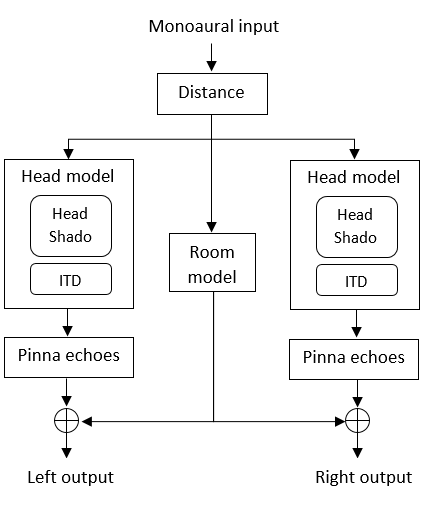
\includegraphics[scale=0.75]{graphics/graphic.png}
	\caption{Components of the model provided on a theoretical basis in~\cite{Brown1997}}
	\label{fig:workflow}
\end{figure}

\begin{figure}[h!]
  \centering
    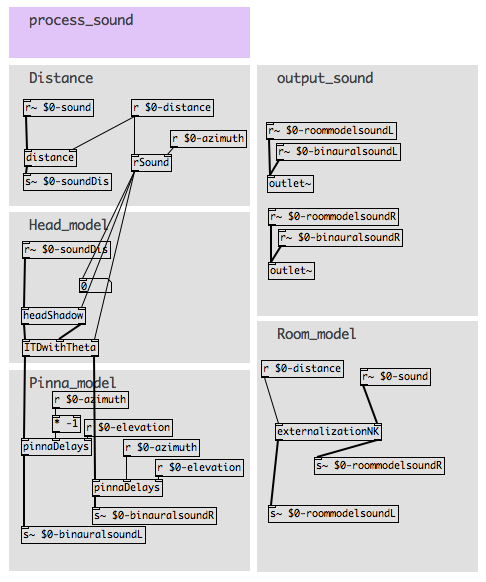
\includegraphics[scale=0.5]{graphics/audioengine.png}
  \caption{The audio engine implemented in Pure Data}
  \label{fig:augioengine}
\end{figure}

To implement the HRTF model~\cite{Brown1997} the audio programming language PureData has been used. Additionaly, in order to embed this model in the Android platform \textit{libpd}\footnote{http://libpd.cc/} has been taken into consideration. Therefore, a PureData external called \textit{headShadow} has been implemented and written in C. Each single part of the HRTF model has been implemented using PureData. 
First, the monoaural sound which has been processed to add a range effect, goes to a head model and a room model. The binaural output of the former is then processed by the pinna model, and finally each one is added to the output of the room model to provide an externalization effect.

In the following formulas, the angles are measured in radians in the interaural-polar system, where $\theta$ is the azimuth angle and $\phi$ is the elevation angle. However, in the mobile application the latter is no considered since all the sound sources are placed in the horizontal plane without elevation.

\subsubsection{The distance model}~\\
In order to simulate the sound pressure in the free field the inverse distance law has been applyed. Since sound intensity is proportional to the square of sound pressure, the inverse square law (for sound intensity) becomes the inverse distance law (for sound pressure)~\cite{everest2009master}. Therefore, sound pressure is inversely proportional to distance \textit{r}:
\begin{equation}\label{eq:soundpressure}
P = \frac{k}{r}
\end{equation}
where \textit{P} is the sound pressure, \textit{k} is a costant and \textit{r} is the distance from source.
Hence, for every doubling of distance \textit{r} from the sound source, sound pressure will be halved. When the distance from
the source is doubled, the sound-pressure level decreases by 6 dB~\cite{everest2009master}.
This model has been implemented in Pure Data.

\subsubsection{The head model}~\\
The path length difference from the sound source to the two ears and the shadowing effect produced by the head at the far ear, lead to a delay and a intensity difference in the sound arriving at the left and right ears. In order to estimate the time delay, the Woodworth's formulas are used~\cite{Woodworth} :

\begin{equation}\label{eq:ITDfront}
ITD = (a/c)[\theta + sin(\theta)]   \; [0 \leq \theta \leq \pi/2]
\end{equation}

\begin{equation}\label{eq:ITDback}
ITD = (a/c)[\pi - \theta + sin(\theta)]  \; [\pi/2 \leq \theta \leq \pi]
\end{equation}


where \textit{a} is the approximated head radius, $\theta$ is the azimuth angle in radians and \textit{c} is the head radius. The time differences between the audio signal reaches the head and the ears are therefore

\begin{equation}\label{eq:ITDL}
T_{L} (\theta) = \frac{a+a\theta}{c}
\end{equation}

\begin{equation}\label{eq:ITDR}
T_{R} (\theta) = \frac{a-a sin(\theta)}{c}
\end{equation}

These formulas refers to a source in front of the head and on the right, with azimuths $0 \leq \theta \leq \pi/2$. If the source is placed on the left ($- \pi/2 \leq \theta \leq 0$), the expressions are reversed.


% We therefore used the analog filter models provided in \cite{Brown1997} and further specified in \cite{Brown1997}.

 % The head shadow filter, implementing the ILD, was given by the following analog transfer function:
 The head shadow effect is characterized in the following analog transfer function:
\begin{equation}\label{eq:analog}
H\left( s,\theta\right) = \frac{\alpha (\theta)s+\beta}{s+\beta},\: where\:\beta = \frac{2c}{a}
\end{equation}


\emph{====Maybe this part in the appendix...?====}

Since this is an analog transfer function we had to derive the digital version by applying a bilinear transform applying the following substitution:

\begin{equation}\label{eq:bilin}
s = \frac{2}{T} \frac{z-1}{z+1},\: where\:T\:is\:the\:sampling\:interval\:in\:seconds
\end{equation}

Applying the substitution in equation~\ref{eq:bilin} to equation~\ref{eq:analog}, we get the following filter function in the digital domain:
\begin{equation}\label{eq:filter}
H\left( z,\theta\right) = \frac{\alpha (\theta)(\frac{2}{T} \frac{z-1}{z+1})+\beta}{(\frac{2}{T} \frac{z-1}{z+1})+\beta}
\end{equation}

To identify the filter coefficients the equation has been transformed ~\ref{eq:filter} and obtained the following frequency response\footnote{For the derivation of Equation~\ref{eq:filterparam} see appendix A}:
\begin{equation}\label{eq:filterparam}
H\left( z,\theta\right) = \frac{2\alpha (\theta)+T\beta+z^{-1}(-2\alpha(\theta)+T\beta)}{2+T\beta+z^{-1}(-2+T\beta)} = \frac{Y(z)}{X(z)}
\end{equation} 

\emph{======================================}

Hence, the filter coefficients $a_0 = 2\alpha (\theta)+T\beta$ and $a_1 = -2\alpha(\theta)+T\beta$ as well as $b_0 = 2+T\beta$ and $b_1 = -2+T\beta$ are given. 
% Since we could not use the filter function in Matlab which has as input values the filter coefficientes we had 
It was necessary to isolate the output $Y(z)$ in Equation~\ref{eq:filterparam} as well as going from the frequency to the time domain. The result is given in Equation~\ref{eq:out}\footnote{For the derivation of Equation~\ref{eq:out} see appendix B}:
\begin{equation}\label{eq:out}
Y[n] =\frac{a_0X[n]+a_1X[n-1]-b_1Y[n-1]}{b_0}
\end{equation} 

\subsubsection{The pinna model}~\\
High frequency components that arrive to the listener's ears are influenced by the pinna, which provide azimuth information. It has been studied mainly because of its contribution to the estimation of the elevation~\cite{Brown1997}.

Our model has the following form:

\begin{figure}[h!]
  \centering
    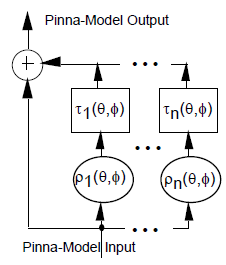
\includegraphics[scale=0.75]{graphics/pinna_part.png}
  \caption{Pinna model. Image taken from~\cite{Brown1997}}
  \label{fig:pinnaModel}
\end{figure}



where the $\rho_{k}$ are the reflection coefficients and the $\tau_{k}$ are the time delays of the \textit{k}th event of a total of \textit{n}. Informal listening tests showed that 5 events were enough to represent the pinna response and that it was convenient to use constant values for the amplitudes $\rho_{k}$,  independent of azimuth, elevation and the subject~\cite{Brown1997}. The time delays seem to be properly approximated by the following formula:

\begin{equation}\label{eq:pinna}
\tau_{k}(\theta,\phi) = A_{k}cos(\theta/2)sin(D_{k}(90\degree-\phi)) + B_{k}
\end{equation} 

In this equation, dependent on the azimuth and elevation, the $A_{k}$ is an amplitude, $B_{k}$ an offset and $D_{k}$ is a scaling factor that should be adapted to the individual listener. 
In the following table one can see the values for the parameters used in the pinna model. Only one set of values for $D_{k}$ in our application have been used.

\begin{table}[h]
\centering
\caption{Pinna model coefficients}
\label{PinnaModel parameters}
\begin{tabular}{|l|l|l|l|l|}
\hline
k & $\rho$  & $A_{k}$ & $B_{k}$  & $D_{k}$   \\ \hline
1 & 0.5   & 1 & 2  & 1   \\ \hline
2 & -1    & 5 & 4  & 0.5 \\ \hline
3 & 0.5   & 5 & 7  & 0.5 \\ \hline
4 & -0.25 & 5 & 11 & 0.5 \\ \hline
5 & 0.25  & 5 & 13 & 0.5 \\ \hline
\end{tabular}
\end{table}



\subsubsection{The room model}
To implement the room model, ask Nikolaj to write something about it.

%\subsection{User interface}
%include pictures of user interface etc.

%%%%%%%%%%%%%%%%%%%%%%%%%%%%%%%%%%%%%%%%%%%%%%%%%%%%%%%%%%%%%%%%%%%%%%%%%%%%%%%%%%%%%%%%%%%%%%%%%%%%%
%%%%%%%%%%%%%%%%%%%%%%%%%%%%%%%%%%%%%%%%%%%%%%%%%%%%%%%%%%%%%%%%%%%%%%%%%%%%%%%%%%%%%%%%%%%%%%%%%%%%%
\section{The experiment}
One of the aims of our experiment was to investigate how fast users were able to locate and navigate to a single sound source using our 3-D audio engine compared to a cosine panner based on~\cite{AndyFarnell2010} and 2/d distance calculation which served as a baseline performance. Therefore the time needed from the beginning of a trial until the sound source was found was measured. 

Additionally we assessed a qualitative analysis of how intuitive it was for subjects to locate the sound as well as investigating whether the sound seemed to be embedded in the real scenery. These results were again compared to the cosine panner model~\cite{AndyFarnell2010}. The data was obtained with a 10 point lickertscale questionnaire going from ``don't agree at all" to `completely agree".

(Here we can write a one paragraph preview of our results.)
%%%%%%%%%%%%%%%%%%%%%%%%%%%%%%%%%%%%%%%%%%%%%%%%%%%%%%%%%%%%%%%%%%%%%%%%%%%%%%%%%%%%%%%%%%%%%%%%%%%%%
%%%%%%%%%%%%%%%%%%%%%%%%%%%%%%%%%%%%%%%%%%%%%%%%%%%%%%%%%%%%%%%%%%%%%%%%%%%%%%%%%%%%%%%%%%%%%%%%%%%%%
\subsection{Materials and methods}
\subsubsection{Participants}
One participant had to be discarded because of 
Qualitative data were collected from 11 participants (3 women and 8 men; mean age: 25, ranging from 22 to 30 years). For the quantitative data 6 more participants were measured summing up to in total 17 participants (4 women and 13 men; mean age: 25, ranging from 22 to 30 years). All participants were students coming from different backgrounds.\footnote{However, 14 subjects were master students in Sound and Music Computing at Aalborg University Copenhagen.} Six students were already familiar with 3-D audio sound and four of them had experience in audio navigation before conduction of the experiment. The other participants were naive. All participants reported normal or corrected to normal vision and no hearing deficits. Participants received no form of compensation other than gratitude. 

\subsubsection{Apparatus and stimuli}
The experiment took place in a free field (grass) in "Valby Parken" in Copenhagen, Denmark (Coordinates: 55$^\circ$38'22.3"N, 12$^\circ$31'27.4"E). The mobile device used was a Motorolla Moto G running with Android version 5.0.2. The device was connected to Sony MDR ZX600 stereo headphones. Only one person at a time was tested. 

To create the auditory stimulus, digital vocal recordings of a male voice (age: ...) were collected using a ... . Recordings were done with ... bits of resolution for amplitude at a sampling rate of ...  kHz. Auditory stimuli were normalized in peak amplitude so that at the minimal distance to the soundsource (7 meter) using the maximal level of volume on the mobile device, the soundlevel of each soundsource was at ... dB. 

\subsubsection{Design}
The experiment comprised one within subject factor at 2 levels (sound engine). The two levels of the sound engine were our 3-D audio engine (3-D) and a cosine panner~\cite{AndyFarnell2010} and distance amplitude modulation (panning).

The starting point was fixed and the distance of the soundsource from that point was always 48 meters.\footnote{However, because of poor GPS accuracies, the location of the soundsource was calculated with the momentary GPS coordinates provided by the phone sensor instead of the actual fixed position in the free field. This ensured that the initial distance to the sound source was always the same.} The sound could appear at any angle from the starting point.

For all trials the same soundfile was played. Each participant performed a total of 6 trials meaning 3 trials in each of the two conditions. Participants were encouraged to take a short break whenever they felt fatigued.

\subsubsection{Procedure}
The position (angle from the starting point) of the sound sources in the different trials were completely randomized within and between subjects independently from the sound engine. This ensured that participants could not predict the location of the sound in the next trial. The order of trials with the one or the other sound engine was not randomized within subjects. Nevertheless, half of the participants started the experiment with the 3-D audio engine while the other half started with the audio panning sound engine to counterbalance for effects related to training. After each block of trials (one block were 3 trials with one of the sound engines) participants had to fill out the qualitative questionaire.

Each trial was initiated by the experimenter with a button press after which the sound source was played. No visual feedback about the location of the sound source or the already passed time to locate it was given. For localization, subjects had to rely solely on the auditory cues given via the headphones. /footnote{Admittedly participants could have used the position of the starting point as some kind of fixpoint. However, participants did know nothing about the possible distances of the sound source. Additionally, questions after the experiment about applied strategies did not reveal that participants used visual cues for localizing the sound source.} As soon as the participants reached a radius of 7 meter around the sound source, an earcon was played indicating the success of the localization. The participants went back to the initial starting point and the next trial was started.

Before the experiment, participants were familiarized with the target sound as well as the earcons that were played when having reached the location of the virtual sound source. Additionally, all participants performed at least two practice trials with the sound engine they were tested with first before the actual measurements with that sound engine began. The location in the practice trials were fixed at the same positions for all participants to allow us to guide the subject when they got lost. 

Participants were instructed to find the sound source as fast as possible. No information about the possible locations (distances and angles) was given to the subjects. Trials which lasted longer than 5 minutes were aborted and labeled as "not found". 

\subsubsection{Analyses}
For the quantitative analysis 26 trials were excluded because either analyses of GPS data for those trials revealed very poor precision (sudden jumps or no changes in the GPS signal for a period of time) or the orientation sensor got stuck which either increased the time needed to find the sound source to a great extent or made it even impossible for the subjects to locate the sound source within 5 minutes. One subject had to be discarded completely from the analyses because there was no single trial with reliable GPS for the panning engine. The other 16 subjects performed at least one trial in each condition. The remaining trials to be analysed summed up to 41 trials in the 3-D condition and 42 trials in the panning condition.

The reasons for choosing a 10 point likertscale instead of the often referenced 5 or 7 point scales~\cite{} were that a greater number of responses should equalize the distances between the possible answer possibilities supporting treating likertscale data also as interval data~\cite{}. This gives us the grounds to use paired samples t-test for the qualitative analysis which is more powefull than the Wilcoxon signed rank test enabling us to detect smaller differences in ratings~\cite{}. Since we only had few questions, having so many answer possibilities should not have fatigued the subject too much so that accuracy of the responses should not have suffered due to too many answer possibilities~\cite{}. Though, it has to be noted that subject were outside when filling out the questionaire which due to cold temperatures might have driven the subjects to respond in a fast pace leading to less accurate responses.

The threshold chosen to correctly reject the null-hypothesis was always 5\% ($\alpha$ = .05).
%%%%%%%%%%%%%%%%%%%%%%%%%%%%%%%%%%%%%%%%%%%%%%%%%%%%%%%%%%%%%%%%%%%%%%%%%%%%%%%%%%%%%%%%%%%%%%%%%%%%%
%%%%%%%%%%%%%%%%%%%%%%%%%%%%%%%%%%%%%%%%%%%%%%%%%%%%%%%%%%%%%%%%%%%%%%%%%%%%%%%%%%%%%%%%%%%%%%%%%%%%%

\subsection{Results}
\subsubsection{Quantitative}
On average subjects needed 104.6 seconds (SD = 44.8) to find the sounds for the 3-D conditions and 109.8 seconds (SD = 44.1) for the panning condition. 

We computed a paired samples t-test to compare the results for both sound engines which revealed no significant difference between the means for both sound engines (t(15) =-.48, p =.64). However, checking whether our data is normally distrubuted using the Shapiro-Wilk test showed that for the 3-D data the assumption of normality was violated (Z=.81, p = .004) and close to significance in the panning condition (Z=.89, p =.054). Therefore, we additionally computed the non-parametric Wilcoxon signed rank test which does not assume normal distributed data. Nevertheless, we could not find a significant difference in scores for time needed to find the soundsource between both conditions (median: 3-D=85.3, panning=95.9; Z=-.83, p = 0.41 ). 

\subsubsection{Qualitative}~\\
The Shapiro-Wilk test showed that the data was normally distributed both for the 3D model (Z = 0.933, p = 0.44) and the Panning model (Z = 0.95, p = 0.67). 

%Statistical tests applied to each question of the questionnaire do not show significant difference between both sound engines either.
Evaluation of the questionnaires, Table \ref{table:questionnairetable}, showed that the mean and median values for questions 1, 2, 3 and 4 for the 3D model were only numerically different from the panning. Neither the paired samples t-test nor the Wilcoxon signed rank test showed significant results comaring the two conditions (3-D vs. panning). However, performing a one sample t-test on means of the four questions for each model comparing it with a neutral response (5.5) showed that users rated the connection between their position and what was presented via the headphones better than neutral for the 3-D sound engine (t(10) = 4.32, p =.002; Z =2.74 , p = .006) but not for the panning (t(10) = 1.07, p = .31; Z = .90, p=.367). For all other questions there were no significant differences.\footnote{It is worth noting that choosing mean and meadian as 5 instead of 5.5, showed that also for question two, a one sample t-test and the wilcoxon signed rank test were significant for the 3-D (t(10) = 2.52 , p = .03 ; Z = 2.19, p =.028) but not for the panning sound engine (t(10) = 1.19, p = .26 ; Z = 1.2, p =.23).}

\begin{table}[h]
\scalebox{0.85}{

 \begin{tabular}{llllllll}

    \toprule
    \multirow{2}{*}{Question} &
      \multicolumn{2}{c}{Mean (s)} &
      \multicolumn{2}{c}{Std (s)} &
      \multicolumn{2}{c}{Median (s)} \\
& {3D model} & {Panning} & {3D model} & {Panning} & {3D model} & {Panning}\\
      \midrule

1    & 6.36    & 5.91    & 1.75    & 1.70    & 6    & 6    \\
2    & 6.91    & 5.82    & 2.51    & 2.27    & 8    & 6    \\
3    & 7.09    & 6.00    & 1.22    & 1.55    & 7    & 6    \\
4\tablefootnote{It should be noted that for this question lower values represent higher quality of a 3-D sound because of the direction of the question.}    & 6.64    & 6.09    & 2.58    & 1.97    & 7    & 5    \\
5    & 6.09    & 6.55    & 2.21    & 2.54    & 7    & 7    \\


    \bottomrule\\
  \end{tabular}\\
  }
  \caption{Questionnaire results}
  \label{table:questionnairetable}
\end{table}

Summing the results for the first four questions to form an overall category of quality of the two sound engines lead to the mean and median values depicted in Table \ref{table:overallquestionaire}. Again, the difference between both sound engines were only numerically visible since performing a paired samples t-test and a Wilcoxon signed rank test showed no significant results  (t(10) = 1.05, p = 0.32; Z = -1.07, p = .283). Furthermore, running a one sample t-test and wilcoxon signed rank test to compare the results of both sound engines to a mean (5.5) that represents being neutral towards a question showed no significant results for both conditions (HRTF: t(10) = 1.54, p = .154; Z = 1.54, p = .13; Panning: t(10) = -.22, p =.829; Z = -0.5, p = .96). However, summing only the first three questions, showed that the 3-D model ratings were significantly higher than the neutral mean (5.5) (t(10) = 2.83, p = .018; Z = 2.09, p = .036) which was not the case for the panning condition (t(10) = .86, p = .41; Z = 0.76, p = .447).

%\begin{verbatim}
%---- Shapiro-Wilk test 3D model ----
%h1 = 0,  p1 = 0.4444,  w1 = 0.9332

% SWstatistic - The test statistic (non normalized).
%
%   pValue - is the p-value, or the probability of observing the given
%     result by chance given that the null hypothesis is true. Small values
%     of pValue cast doubt on the validity of the null hypothesis.
%
% The null-hypothesis of this test is that the population is normally distributed
%     H = 0 => Do not reject the null hypothesis at significance level ALPHA.
%     H = 1 => Reject the null hypothesis at significance level ALPHA.

%
%---- Shapiro-Wilk test panning ----
%h2 = 0,  p2 = 0.6878,  w2 = 0.9534
%
%---- perform paired samples t-test ----
%ht_test = 0
%pt_test = 0.3199
%ci = [-2.3598 6.5417]
%
%statst_test = 
%    tstat: 1.0468
%       df: 10
%       sd: 6.6250
%
%---- perform Wilcoxen-signed rank test ----
%p = 0.3223
%h = 0
%stats = signedrank: 38
%\end{verbatim}


\begin{table}[h]
\scalebox{0.85}{
 \begin{tabular}{llllllll}

    \toprule
    \multirow{2}{*}{Question} &
      \multicolumn{2}{c}{Mean (s)} &
      \multicolumn{2}{c}{Std (s)} &
      \multicolumn{2}{c}{Median (s)} \\
%& {model 1} & {model 2} & {model 1} & {model 2} & {model 1} & {model 2}\\
& {3D model} & {Panning} & {3D model} & {Panning} & {3D model} & {Panning}\\
      \midrule

1 - 4      & 5.93  & 5.41  & 0.93    & 1.36    & 6  & 5.25\\

    \bottomrule\\
  \end{tabular}\\
  
  }
  \caption{Overall results}
\label{table:overallquestionaire}
\end{table}

\section{Discussion}
The results show that both sound engines did not differ in terms of performance. Although numerically subjects were slightly faster to locate the sound source when using the HRTF audio engine, this difference could not be verified statistically.\footnote{However, it might have been the case that our sample size was so small that the difference in performance would have had to be bigger to show significant results given the sample size in this experiment. As noted by several methodologists Type II errors have a high probability to occur for low sample sizes \cite{DeWinter2013}}.  

As for the qualitative analyses the explanation why our 3-D audio engine was not rated significantly better then the other could be due to the choice of a unnatural high reverberation level for a free field. This explanation is inspired by the fact that a lot of participants had background knowledge in acoustics and therefore made more predictions about a proper reverberation level for a free field. Some subjects even reported the reverberation to be the reason for low ratings of the question regarding whether the soundsource was perceived to be embedded in the real scenery. This negative effect on the ratings might have nullified the difference between panning and HRTF in terms of perceiving the sound moving around and not inside the head. Some support for this explanation can be gained from noticing that the ratings of the first three questions taken together (as well as the third question alone) were significantly higher than a neutral response for the HRTF but not for the Panning. This might illustrate a slight superiority in quality of the HRTF.

Another issue that should be adressed is the adequacy of the questionaire used in this experiment. Probably, in spite of the discussion about why we chose to use a 10-point likert scale instead of the often used 5- or 7-point likert scale, subjects might not have been able to accurately respond to the questions posed leading indistinguishable results. Also the fact that most of the questions were not different to the mean of the scale provide some evidence that subjects were either actually indifferent to the posed questions or had difficulties of knowing which number corresponds to which degree of agreement to the stated question.

%%%%%%%%%%%%%%%%%%%%%%%%%%%%%%%%%%%%%%%%%%%%%%%%%%%%%%%%%%%%%%%%%%%%%%%%%%%%%%%%%%%%%%%%%%%%%%%%%%%%%
%%%%%%%%%%%%%%%%%%%%%%%%%%%%%%%%%%%%%%%%%%%%%%%%%%%%%%%%%%%%%%%%%%%%%%%%%%%%%%%%%%%%%%%%%%%%%%%%%%%%%

\section{Conclusion}


\section{Future works}

% conference papers do not normally have an appendix


% use section* for acknowledgment
\section*{Acknowledgments}






% \begin{thebibliography}{4}

% \bibitem{Brown1997}
% C. Phillip Brown and Richard O. Duda, \textit{An efficient HRTF model for 3-D sound}. Proceedings of the IEEE Workshop on Applications of Signal Processing to Audio and Acoustics. New York: IEEE. 1997

% \bibitem{HowTo}Johannes M. Zmoelnig, \textit{HOWTO write an External for puredata}.\\\texttt{ http://
% pdstatic.iem.at/externals-HOWTO/}, 2010.

% \bibitem{Woodworth}Neil L. Aaronson and William M. Hartmann, \textit{Testing, correcting, and extending the Woodworth model
% for interaural time difference}. Acoustical Society of America, 2014.

% \bibitem{AnalysingLop} P.M. Delgado. \textit{First steps on Pure Data’s approach to real time audio processing. Compiling externals. Analysing lop~}. https://pmdelgado.wordpress.com/2015/09/17/first-steps-on-pure-datas-approach-to-real-time-audio-processing-compiling-externals-analysing-lop/



% \end{thebibliography}


% trigger a \newpage just before the given reference
% number - used to balance the columns on the last page
% adjust value as needed - may need to be readjusted if
% the document is modified later
%\IEEEtriggeratref{8}
% The "triggered" command can be changed if desired:
%\IEEEtriggercmd{\enlargethispage{-5in}}

% references section

% can use a bibliography generated by BibTeX as a .bbl file
% BibTeX documentation can be easily obtained at:
% http://mirror.ctan.org/biblio/bibtex/contrib/doc/
% The IEEEtran BibTeX style support page is at:
% http://www.michaelshell.org/tex/ieeetran/bibtex/
%\bibliographystyle{IEEEtran}
% argument is your BibTeX string definitions and bibliography database(s)
%\bibliography{IEEEabrv,../bib/paper}
%
% <OR> manually copy in the resultant .bbl file
% set second argument of \begin to the number of references
% (used to reserve space for the reference number labels box)
%\begin{thebibliography}{1}
%
%\bibitem{IEEEhowto:kopka}
%H.~Kopka and P.~W. Daly, \emph{A Guide to \LaTeX}, 3rd~ed.\hskip 1em plus
%  0.5em minus 0.4em\relax Harlow, England: Addison-Wesley, 1999.
%
%\end{thebibliography}

\pagebreak
\listoffigures
\listoftables
\pagebreak
\begin{appendices}
\section{Derivations}
\begin{equation*}\label{eq:DerivationFilterCoeff}
\begin{split}
H\left( z,\theta\right) &=\frac{\alpha (\theta)(\frac{2}{T} \frac{z-1}{z+1})+\beta}{(\frac{2}{T} \frac{z-1}{z+1})+\beta}\\
                                   &= \frac{\frac{2\alpha (\theta)(z-1)}{T(z+1)}+\frac{T\beta(z+1)}{T(z+1)}}{\frac{2(z-1)}{T(z+1)}+\frac{T\beta(z+1)}{T(z+1)}}\\  
			   &=\frac{\frac{2\alpha (\theta)(z-1)+T\beta(z+1)}{T(z+1)}}{\frac{2(z-1)+T\beta(z+1)}{T(z+1)}}\\
			  &=\frac{2\alpha (\theta)(z-1)+T\beta(z+1)}{2(z-1)+T\beta(z+1)}\\
			 &=\frac{z2\alpha (\theta)(1-z^{-1})+zT\beta(1+z^{-1})}{z2(1-z^{-1})+zT\beta(1+z^{-1})}\\
			&=\frac{2\alpha (\theta)(1-z^{-1})+T\beta(1+z^{-1})}{2(1-z^{-1})+T\beta(1+z^{-1})}\\
			&=\frac{2\alpha (\theta)-2\alpha (\theta)z^{-1}+T\beta+T\beta z^{-1}}{2-2z^{-1}+T\beta+T\beta z^{-1}}\\
			&=\frac{(2\alpha (\theta)+T\beta)-(2\alpha (\theta)+T\beta)z^{-1}}{(2+T\beta)-(2+T\beta)z^{-1}}\\
			&=\frac{(2\alpha (\theta)+T\beta)+(-2\alpha (\theta)+T\beta)z^{-1}}{(2+T\beta)+(-2+T\beta)z^{-1}}\\
\end{split}
\end{equation*} 
\section{Derivations}
\begin{equation*}\label{eq:DerivationC++}
\begin{split}
H(z, \theta) &= \frac{Y(z)}{X(z)} = \frac{a_0+a_1z^{-1}}{b_0+b_1z^{-1}}\\
&\iff Y(z)(b_0+b_1z^{-1}) = X(z)(a_0+a_1z^{-1})\\
&\iff Y(z)b_0+b_1Y(z)z^{-1} = a_0X(z)+a_1X(z)z^{-1}\\
&\iff Y(z) = \frac{a_0X(z)+a_1X(z)z^{-1}-b_1Y(z)z^{-1}}{b_0}\\
&\rightarrow Y[n] = \frac{a_0X[n]+a_1X[n-1]-b_1Y[n-1]}{b_0}
\end{split}
\end{equation*} 
\end{appendices}

\pagebreak
% Style and bibliography.
% The bibtex filename
%bliography{}
% \section*{References}
\bibliographystyle{ieeetr}
\bibliography{biblio}

% that's all folks
\end{document}


